%%%%%%%%% MASTER -- compiles the 4 sections

\documentclass{article}
\usepackage{graphicx}
\usepackage{xr}
\usepackage{subcaption}
\def\baselinestretch{1}
%%%%%%%%%%%%%%%%%%%%%%%%%%%%%%%%%%%%%%%%%%%%%%%%%%%%                                   
\newcommand{\required}[1]{\subsection*{\hfil #1\hfil}}          
\renewcommand{\refname}{\hfil References Cited\hfil}         
%\bibliographystyle{mrsnsf}
%\bibliographystyle{acm}
\bibliographystyle{apsrev}
%   Use the command \bibpunct with one optional and 6 mandatory arguments: 
%   1. the opening bracket symbol, default = (
%   2. the closing bracket symbol, default = )
%   3. the punctuation between multiple citations, default = ;
%   4. the letter `n' for numerical style, or `s' for numerical superscript style, any other letter for author-year, default = author-year;
%   5. the punctuation that comes between the author names and the year
%   6. the punctuation that comes between years or numbers when common author lists are suppressed (default = ,);
%\bibpunct{}{}{,}{s}{}{,}
%\bibpunct{(}{)}{;}{a}{}{,}
%%%%%%%%%%%%%%%%%%%%%%%%%%%%%%%%%%%%%%%%%%%%%%%%%%%

%PUT YOUR MACROS HERE
\usepackage[colorlinks=true,citecolor=blue,linkcolor=blue]{hyperref}

%\includeonly{NSFsumm}
\newcommand{\Var} [1]{\mathrm{var}{\left(#1\right)}}
\newcommand{\Cov}[1]{\mathrm{Cov}{\left(#1\right)}}
\newcommand{\ens}[1]{\left \langle #1 \right \rangle}
\newcommand{\dhdl}{\frac{dH}{d\lambda}}
\newcommand{\smallhead}[1]{\noindent {\em #1}:} 
\newcommand{\vx}{\mathbf x}
\begin{document}
% The figures are in a figures/ subdirectory.
\graphicspath{{figures/}}
%%%%%%%%% PROPOSAL -- 10 pages maximum 

% use letters for the subsections with this command
\def\thesection{\Roman{section}.}
\def\thesubsection{\alph{subsection}.} 
\def\thesubsubsection{\alph{subsection}.\roman{subsubsection}}
\subsection{How do water and ions move in nanostructured charged polymeric membranes?}
\subsubsection*{Background} 

The ability to design nanostructured membranes with concomitant high chemical
specificity is an important goal of the membrane separations
community.~\cite{Humplik2011} The ability to control
the nanoscale architecture of membranes will allow membranes to be 
designed precisely for the purpose of separating specific compounds.
~\cite{SmithRC1997,Zhu2006} The membranes being studied in this project
have pores sizes smaller than 1 nanometer, allowing size-selective 
filtration of small molecules and gases, as well as desalination of salt
water based on charge repulsion and size-exclusion of hydrated salt ions.

The membrane system we propose to model in this project is composed of
lyotropic liquid crystals (LLCs) which self-assemble into hexagonally
packed, cylindrical pores with acidic groups facing toward the cylinder
center, complexed to counterions. Subsequent cross-linking of vinyl
groups on monomer tail ends forms a mechanically strong structure
(Fig.~\ref{figure:membrane}). ~\cite{Zhou2003,Feng2014,Feng2016}
The pores, at the level of resolution obtained by SAXS and TEM, appear
to be straight and uniform in size (Fig.~\ref{figure:membrane}). 
This is very different from most commercially available membranes 
which have a pore size distribution with tortuous pathways that reduce
selectivity and flux respectively. The ordered structure exhibited by
LLC membranes makes them well suited for modeling using molecular 
dynamics simulations because the system has a defined structure that
can be studied in detail with a reasonably sized unit cell.

Our initial systems were built by first parameterizing a single
monomer using the General Amber Force Field (GAFF). Because the
self-assembly process is long relative to times which we can simulate,
monomers were rotated into layers of six monomers and stacked into
cylinders to give a starting configuration close to where we expect
the system to settle at equilibrium. While a single lyotropic liquid
crystal consists of a small number of atoms (138), the entire unit
cell consists of about 66K atoms. This number increases to 
approximately 100K when water molecules are added to the system.

Equilibration simulations have been performed which energy minimize and
allow the system to stabilize over the course of 500 ns in vacuum.  The
final structure and trajectory are analyzed quantitatively by
measuring pore size, distance between pores, distribution of
sodium ions in the pore, simulating X-ray diffraction patterns and 
calculating ionic conductivity. These measurements are compared to values
measured experimentally with SAXS and TEM imaging in order to validate
the final structure. SAXS and TEM images were taken using dry membrane
which justifies our initial study of the system in vacuum.

\begin{figure}[h]
\begin{center}
\begin{tabular}{c}
\includegraphics[width=8cm]{modeled.png}\\
\includegraphics[height=5cm]{membraneviews.png}\\
\end{tabular}
\end{center}
\caption{(above) SAXS and TEM experimental data, with hypothesized
  membrane structure. (Below, left) Top view of atomistic simulation,
  with hydrophilic head groups in orange, counterions in blue, and
  hydrophobic chains in blue. (Below, right) Side view of atomistic
  simulation showing counterions in dark blue and other atoms in light
  blue. These simulations demonstrate the heterogeneity in the
  modeled systems.~\label{figure:membrane}}
\end{figure}

\subsubsection*{Proposed Experiments and Justification of Resources}

Vacuum simulations of this system with a unit cell consisting of 4
pores, each with twenty layers of six monomers, total 66K atoms. On
Bridges, using MPI-enabled GROMACS 5.1.2, we obtain
99 ns/day using 224 cores, beyond which the scaling becomes mildly
nonlinear (See Figure~\ref{figure:gromacs} in the ``Code Performance
and Scaling'' document for more details). Simulations of the same
system solvated in water results in a total of 100K atoms, which ran
at 121 ns/day using 336 cores, at the limit of the near linear scaling
regime.  By creating a system with 80 layers, we reached 265K atoms,
which scaled nearly linearly up to 29 ns/day on 224 cores. We will use
these timings to estimate the time required for these experiments.

We repeated scaling studies with the same systems using GPU-enabled 
GROMACS 2016 with both the NVIDIA K80 and NVIDIA P100 GPUs available on
Bridges. Using 4 K80 GPUs we obtain 58 ns/day, 56.4 ns/day and 10.1 ns/day
for the 66K, 100K and 256K atom systems respectively. Although the system
scales nearly linearly for greater than 4 GPUs in all cases, additional
GPUs require more than 1 node which has signficantly extended queue wait
times in our experience. It is preferable to run jobs longer on one GPU
for a long time than to delay a job from starting but have it run for a
shorter time. Since trajectory files are written while simulating, it
is beneficial to check progress and cancel jobs which show no value.
We plan to work with PSC to compile a version of gromacs that is performs
optimally with the
 

In order to study the relative stability of the two metastable phases 
we have discovered, we will need to perform a computationally 
intensive free energy calculation using the Multistate Bennett
Acceptance Ratio (MBAR) technique. MBAR estimates free energy 
differences with the currently lowest variance when compared to other
estimators. In order to make a reasonable estimate, we will need to 
conduct simulations of all intermediate states which lead from one metastable
state to another. Each configuration in the pathway mapping the two
states must be sufficiently similar to adjacent configurations so that
we achieve enough phase space overlap for a more precise calculation. 
We estimate that we will need at least 50 intermediate states, each run
for 50 ns for a total of 2500 ns of simulation time. This will require 
(2500 ns / (99.2 ns/day))* 24 hrs/day * 224 cores = 135K SU using
MPI on the RM partition. This will require (2500 ns / (58 ns/day)) * 24
hours * 4 GPUs = 4.1K SU on the K80 GPU nodes.

The resolution of simulated X-ray diffraction patterns is dependent on the
size of the simulated unit cell. To create higher resolution patterns in 
the x, y or z directions, requires an increase in the respective dimension
of the unit cell by adding more atoms. The fundamental reason for this
limitation is the necessity of meeting the Bragg condition. When met,
constructive X-ray interference occurs resulting in a signal which gives
details about the position of atoms relative to each other. The lattice
planes in the crystal, defined by the reciprocal space Miller indices 
h, k, and l, are separated by a distance, d. One can calculate all possible
d values given all unit cell parameters. It is not trivial to see that an
increase in box vector leads to a wider range of accessible hkl values 
and increases the spatial resolution. A simple way to estimate the simulated
resolution in each direction is using the equations qx = 2*pi/x, qy = 2*pi/y,
qz = 2*pi/z. Our current resolution with a 66K atom system is ~ 0.078 inverse
angstroms (Fig.~\ref{fig:expxrdcomp}). We propose a 4x increase in our z dimension resolution which will
help us to distinguish reflections deemed a consequence of benzene ring 
pi-stacking (reflection occurs at 1.53 inverse angstroms) from simple
alkane chain packing (reflection occurs between 1.4 and 1.57 inverse
angstroms). We also hope to pick up finer details such as the sharp line
that appears at ~.85 inverse angstroms experimentally but is absent in 
the simulated patterns. A system of this size is made of 265K atoms. 
Stacking equilibrated membrane layers directly on top of each will 
facilitate a fast equilibration of the large system. Equilibration 
simulations will be run for at least 50 ns followed by another 50 ns of 
simulation needed to collect enough information to simulate the XRD 
pattern. 100 ns of simulation time for a 265K atom system will require 
19K SU on the RM nodes and 950 SU on K80 GPU nodes.     

\begin{figure}
\centering
\includegraphics[width=\linewidth]{Sim_exp_xrd_sidebyside.png}
	\caption{(left) Experimental Wide Angle X-ray Diffraction experiments contain
reflections at qz \approx 1.7 A $^{-1}$ indicating pi-stacking of benzene
rings in the monomer head group. A weak, correlated reflection is present at 
qz \approx 0.85 A $^{-1}$. (right) Simulated X-ray diffraction shows a pi-stacking reflection
at qz \approx 1.5 A $^{-1}$. The weak correlated reflection is not
present but may be visible with higher resolution simulations}
	\label{fig:expxrdcomp}

\end{figure}

Once equilibrated and cross-linked, we will examine the effect of membrane
solvation on the pore structure and corresponding transport properties.
We have learned that at least 1000 ns of total simulation is required
to fully equilibrate the system with water. (1000 ns / (86 ns/day)) * 24
hours * 224 cores = 62K required SU, if we assume the initial
membrane simulation boxes are sufficiently large.

We will carry out the same procedure with a new set of monomers similar
in structure to the current monomer. Simple modifications can be made
to the monomer structure as outlined in Figure ~\ref{fig:chemistries}. 
We will need to equilibrate each system using developed procedures which
requires equilibration simulations of at least 500 ns. Of the 
possibilities outlined in Figure ~\ref{fig:chemistries} we will try all
variations of tail spacer and ionic headgroup and at least 3 counterions
of different charge (+1, +2, +3). This results in a total of 24 systems 
that require 500 ns of equilbration time. These length simulations should
also give us the required information to calculate physical properties 
such as ionic conductivity, and to simulate X-ray diffraction patterns.
We will require xxx SU explore this space. To solvate all the test
systems, an additional xxx SU will be necessary.

We will conduct transport studies on all systems in order to relate pore
structure to macroscopic observables such as water flux and solute
rejection. We will measure diffusion of various solutes across the 
membrane. Understanding the mechanims of transport of each solute will
provide us with sufficient understanding to suggest new modifications 
to monomer structure that should increase laboratory performance. We
anticipate simulations of at least 50 ns will be necessary to get 
sufficient sampling for an informative mean square displacement (MSD) 
curve. The MSD curve will make it easier to identify potential 
transport mechanisms based on its shape.

\begin{figure}
\centering
\includegraphics[width=\linewidth]{chemistries.png}  % who made this picture? It has a typo : "ionic headgoup"
	\caption{LLC chemistries we will examine in order to understand determinants of pore size, structure and solute transport}
	\label{fig:chemistries}
\end{figure}

%\begin{wraptable}{r}{0.4\textwidth} 
%\begin{tabular}{|l|c|}
%\hline
%Simulation Set                & SU \\ 
%\hline
%Initial vacuum equilibration      &  57K \\
%Test of monomer structuring       & 114K \\
%System-size dependence            & 102K  \\
%Membrane solvation                &  375K \\
%Diffusion studies                 & 72K \\
%Differences in bound counterion  & 430K \\
%\hline
%            Total         & 1140K \\
%\hline
%\end{tabular}


\newpage
%bibliography
\bibliography{teragrid,ReweightingValidationPaper}{}
\newpage
\include{scaling}
\newpage
\section*{Summary of Scientific Discoveries}

\subsection*{Simulations of transport in nanostructured polymer membranes}
Our understanding of the microscopic structure of this type of LLC
membrane has greatly increased with the aid of simulations run using
Bridges. 

Equilibration simulations of greater than 500 nanoseconds yield
stable membrane configurations with the expected HII phase 
morphology. Various methods have been developed to characterize
the equilibrated system. Generally, all equilibrium properties are
compared to experimental measurements. We validated two methods
for measuring ionic conductivity from atomistic simulations. Both 
methods require long simulations (at least 500 ns) in order to give
accurate statistics. The distance between pores is an important
structural parameter which we have measured using atomic coordinates
and by simulating X-ray diffraction (XRD) experiments, a relatively
undeveloped technique in MD for periodic systems such as ours. We 
have been able to generate structures which match experimental pore
spacings within reason.

The X-ray diffraction simulations also give detailed information
about membrane structure on the angstrom lengthscale. Our simulations
have produced two dimensional X-ray diffraction patterns that 
contain all major features present in experimental studies. Producing
a matching pattern was not trivial and resulted in the discovery of
two metastable states. The two states are defined by the degree of 
local order inside the pore regions. The state which we had initially
studied is characterized by a disordered pore region, however the X-ray
diffraction pattern does not match experiment. We altered the starting 
configuration so that the benzene rings in the head group of each
monomer were stacked in a parallel displaced configuration relative
to each other. The resulting X-ray diffraction pattern of the new
configuration, after equilibration, is a much closer match to experiment.
Additionally, we were able to explain the spots that appear (red arrows
in figure xx) contrary to how it was originally reported. The spots 
were assumed to be caused by the 40 degree tilt angle of the alkyl
tails with respect to the plane of each stacked monomer layer, a 
common feature of liquid crystal systems. However, we were able to 
produce the same spots using configurations with an average tilt angle
close to zero. Our most impactful finding remains as the discovery of 
two metastable states. This will be the subject of a publication which 
will be submitted in the coming months. In the future, we will conduct
free energy calculations that will help explain the difference between
the two states and and help predict what experimental conditions might
lead to each. 

\begin{figure}
\caption{}
\label{figure:metastable}
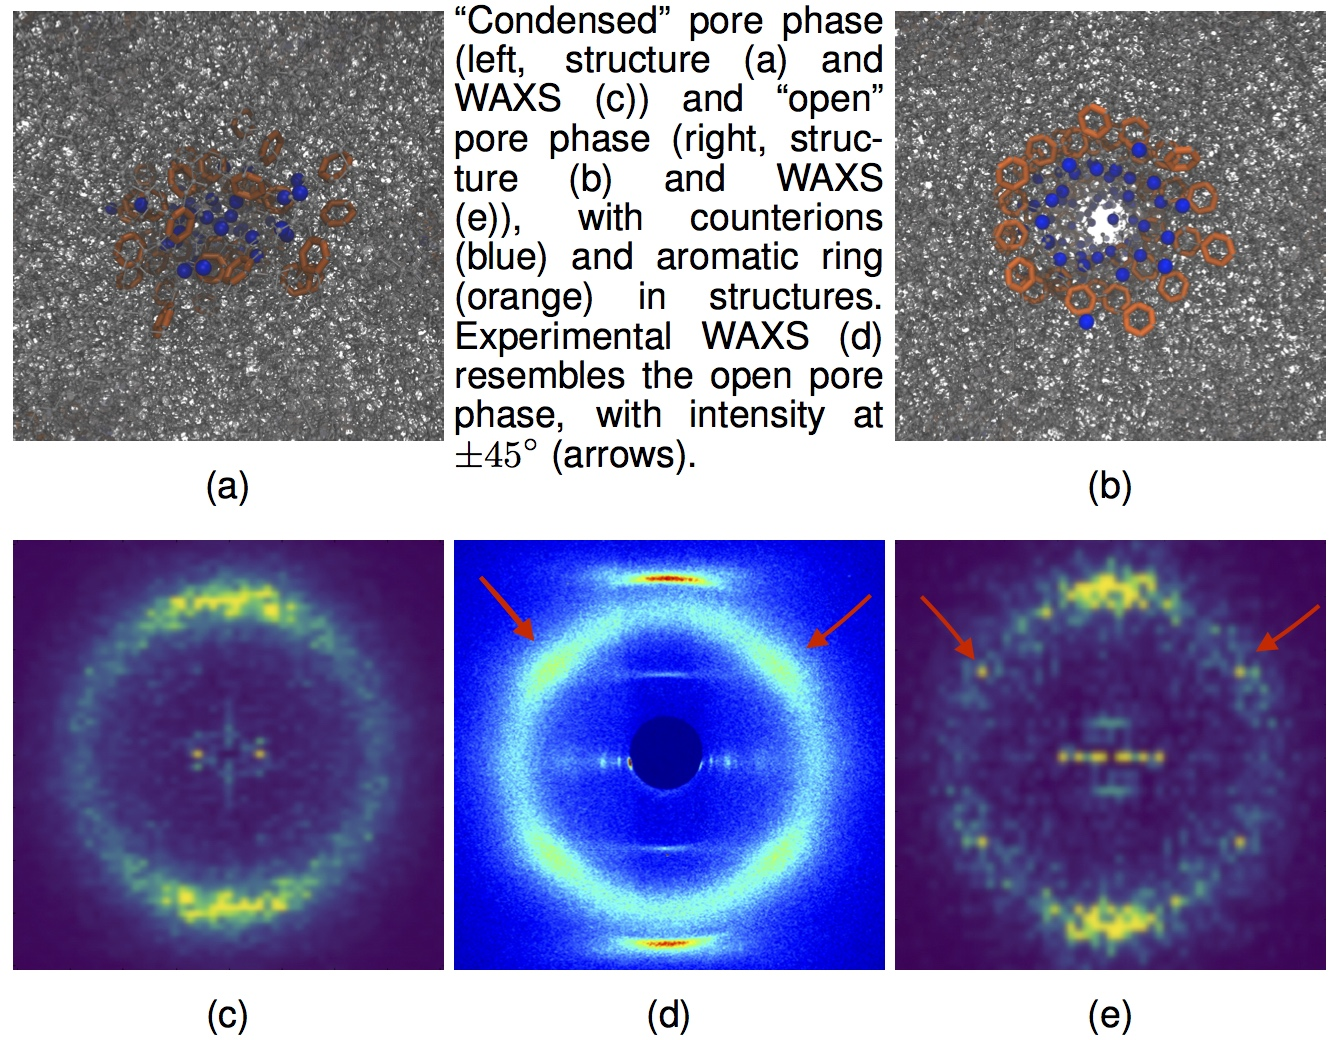
\includegraphics[width=.9\textwidth]{porestructures.jpg}
\centering
\end{figure}

The next step for our system is to solvate it with water. In parallel 
to the preceding work, we have worked to develop methods which will be
used to study the solvated system. While measuring ionic conductivity 
and running XRD simulations will work just the same, equilibration is 
non-trivial. We do not know exactly the equilibrium content of water 
or where the water is situated. While it is clear that most water should be in the hydrophilic pore region, simulations have shown that an 
appreciable amount of water can exist in the tail region near the 
slightly hydrophilic ester group. The best way to figure out how much 
water should be in the pore is to run very long equilibration simulationsand allow the simulations to tell us. Our current approach is to create
water baths at each face of the membrane and allow water to diffuse into
the membrane. We have learned that we can equilibrate a membrane with
water in 1000 nanoseconds. Studies of the hydrated, 'lyotropic', phase
will be the subject of a subsequent publication.


\end{document}
